\documentclass{cours}
\usepackage{esvect}
\usepackage{pgfplots}
\usepackage{multicol}
\usepackage{mathrsfs}
\usepackage{amssymb}
\usepackage{tikz-3dplot}
\usepackage{xr}
\usepackage{fontawesome}
\usetikzlibrary {decorations.text, backgrounds, intersections}

\begin{document}

\newcommand{\cc}{\ensuremath{\mathscr{C}}}

\setcounter{chapter}{25}
\chapter{Circuit fixe dans un champ magnétique variable}
\section{Auto-induction}%
\label{sec:auto_induction}

\subsection{Flux propre et flux extérieur}%
\label{sub:flux_propre_et_flux_exterieur}
Soit $\Phi$ le flux total du champ magnétique à travers un circuit \cc. On peut décomposer $\Phi$ en deux contributions : 
\begin{equation}
  \Phi = \Phi_p + \Phi_e
\end{equation}
\begin{itemize}
  \item $\Phi_p$ est le flux propre, c'est le flux à travers \cc du champ magnétique créé par \cc ;
  \item $\Phi_e$ est le flux extérieur, c'est le flux à travers \cc du champ créé par d'autres sources que \cc.
\end{itemize}

\subsection{Auto-induction}%
\label{sub:auto_induction}
 
On considère que le champ magnétique est uniquement produit par le circuit \cc, le flux du champ à travers \cc sera donc le flux propre $\Phi = \Phi_p$. Lorsque le flux varie à travers \cc, il apparait une fem induite dans le circuit \cc
\begin{equation}
  e = -\dt{\Phi}
\end{equation}
Or, le champ magnétique produit par \cc est proportionnel au courant $i$ qui circule dans \cc, donc le flux $\Phi$ sera aussi proportionnel à $i$.  On peut écrire 
\begin{equation}
  \Phi = Li
\end{equation}
La constante de proportionnalité $L$ est l'\textbf{inductance propre} du circuit. Elle ne dépend que des caractéristiques géométriques du circuit. Dans ces conditions, on aura
\begin{equation}
\label{eq:autoinduction}
e = -L\dt{i}
\end{equation}
On retrouve la loi qui relie la tension aux bornes d'une bobine à l'intensité du courant qui la traverse. 

\textbf{Attention : } l'équation~\ref{eq:autoinduction} comporte un signe "$-$" qui vient d'une orientation différente de la tension d'une bobine et de la fem induite
\begin{center}
  \begin{tikzpicture}
    %tikz induction
    \draw (0,0) to[L, v=$u$, i=$i$] (3,0);  
    \draw (1.5, -0.5) node[below]{Bobine};
    \draw (6,0) to[european voltage source, v=$e$] (8,0) to[short, i=$i$] (8,2) to[short] (6,2) to[short] (6,0);
    \draw (7, -0.5) node[below]{Induction};
  \end{tikzpicture}
\end{center}
\begin{application}
 Dans une bobine longue (solénoïde) de longueur $\ell$, comportant $N$ spires, le champ magnétique peut être considéré comme uniforme et vaut 
 \begin{equation}
   \vv{B} = \mu_0 n i \vez\,,
 \end{equation}
 avec $n=N/\ell$ le nombre de spires par mètre de la bobine et $\vez$ orienté suivant l'axe de la bobine. Le flux du champ magnétique à travers une spire est $\Phi_1 = BS$, avec $S$ la surface d'une spire. Le flux total à travers la bobine est
 \begin{equation}
   \Phi = N\Phi_1 = \frac{\mu_0N^2Si}{\ell}
 \end{equation}
 On en déduit l'expression de l'inductance $L$ de la bobine : 
 \begin{equation}
 \label{eq:L}
   L = \frac{\mu_0 N^2S}{\ell}
 \end{equation}
\end{application}


\subsection{Aspect énergétique}%
\label{sub:aspect_energetique}
On considère un circuit électrique dans lequel se produit un phénomène d'auto-induction :
\begin{center}
\begin{tikzpicture}
  \draw (0,0) to[european voltage source, v=$E$ ] (0,2) to[european resistor, l=$R$, i=$i$] (3,2) to (3,1.2) -- ++(0.5, 0) arc({180-atan(0.2/0.7)}:{-180+atan(0.2/0.7)}:0.7) -- ++(-0.5, 0) -- (3,0) -- (0,0);
  \draw[-latex]  (2.7, 1.5) -- (2.7, 0.5) node[midway, left] {$e$};
  \draw[decorate, decoration={brace, mirror}] (3.5, 0.1) -- (4.9, 0.1) node[midway, below]{Auto induction};
\end{tikzpicture}
\end{center}
La loi des mailles dans ce circuit donne 
\begin{equation}
  E = Ri -e = Ri+L \dt{i}
\end{equation}
La puissance fournie par le générateur est
\begin{equation}
  P=Ei = \underbrace{Ri^2}_{P_J} + \underbrace{Li \dt{i}}_{P_S}
\end{equation}
$P_J$ est la puissance dissipée par effet Joule dans la résistance et $P_S$ est la puissance stockée dans le champ magnétique. On a 
\begin{equation}
P_S = Li \dt{i} = \dt{}\underbrace{\left[ \frac{1}{2} Li^2\right] }_{E_m}
\end{equation}
$E_m$ est l'énergie stockée sous forme de champ magnétique dans le circuit. On en déduit que lorsqu'un circuit d'inductance propre $L$ est parcouru par un courant $i$, il stocke une énergie 
\begin{eqencadre}
  E_m = \frac{1}{2}Li^2
\end{eqencadre}
\section{Inductance mutuelle}%
\label{sec:inductance_mutuelle}

\subsection{Interaction entre deux bobines}%
\label{sub:interaction_entre_deux_bobines}
On considère deux circuits $\cc_1$ et $\cc_2$ parcourus par des intensités $i_1$ et $i_2$ et dans lesquels il existe des fem induites $e_1$ et $e_2$. 

\begin{minipage}{\linewidth}
\begin{center}
  \begin{tikzpicture}
    %tikz induction
    \draw[postaction={decorate, 
    decoration={markings,
    mark=at position 0.1 with{\arrow{latex};\draw (0,0) node[right] {$i_1$}; }}}
    ] (0,0) ellipse[x radius=0.7, y radius=1.5];
    \draw (0.7, 0) circle(0.3);
    \draw[-latex] (1.1, -0.3) -- (1.1, 0.3) node[midway, right]{$e_1$} ;
    \draw (0,0) node{$\mathscr{C}_1$}; 

    \begin{scope}[xshift=4cm]
    \draw[postaction={decorate, 
    decoration={markings,
    mark=at position 0.1 with{\arrow{latex};\draw (0,0) node[right] {$i_2$}; }}}
    ] (0,0) ellipse[x radius=0.7, y radius=1.5];
    \draw (0.7, 0) circle(0.3);
    \draw[-latex] (1.1, -0.3) -- (1.1, 0.3) node[midway, right]{$e_2$} ;
    \draw (0,0) node{$\mathscr{C}_2$}; 
    \end{scope}
  \end{tikzpicture}
  \captionof{figure}{Deux circuits où se produit un phénomène d'induction}
\end{center}
\end{minipage}
Dans ce cas, le champ magnétique total $\vv{B}$ est la somme des champs magnétiques $\vv*{B}{1}$ et $\vv*{B}{2}$ produits par les circuits $\cc_1$ et $\cc_2$. On peut décomposer le flux de $\vv{B}$ à travers le circuit $\cc_1$ comme 
\begin{equation}
  \Phi_1 = \Phi_{1\rightarrow 1} + \Phi_{2\rightarrow 1}
\end{equation}
\begin{itemize}
  \item $\Phi_{1\rightarrow 1}$ est le flux du champ $\vv*{B}{1}$ à travers $\cc_1$. Il est donné par $\Phi_{1\rightarrow 1} = L_1i_1$.
  \item $\Phi_{2\rightarrow 1}$ est le flux du champ $\vv*{B}{2}$ à travers $\cc_1$. Comme $\vv*{B}{2}$ est proportionnel à $i_2$, on a $\Phi_{2\rightarrow 1} = M_{21}i_2$.   
\end{itemize}
Dans ces conditions, on a 
\begin{equation}
  e_1 = -\dt{\Phi_1} = -\dt{\Phi_{1\rightarrow 1}} -\dt{\Phi_{2\rightarrow 1}}
\end{equation}
Soit
\begin{eqencadre}
   e_1 = -L_1 \dt{i_1} - M_{21}\dt{i_2}
\end{eqencadre}
et de la même manière, on trouve 
\begin{eqencadre}
  e_2 = -L_2\dt{i_2} - M_{12} \dt{i_1}
\end{eqencadre}

On peut montrer que $M_{12} = M_{21} = M$ et on appelle cette quantité l'\textbf{inductance mutuelle} entre les deux circuits.  

\textbf{Attention : } l'inductance mutuelle peut être positive ou négative, contrairement à l'inductance propre qui est toujours positive. Le signe de l'inductance mutuelle dépend de l'orientation choisie pour les deux circuits. 

\begin{application}
  On considère deux solénoïdes de même section, de même longueur, coaxiaux. Le premier solénoïde comporte $N_1$ spires et le second en comporte $N_2$. 

  Le champ magnétique produit par un solénoïde de longueur $\ell$ comportant $N$ spires est $\vv{B} = \frac{\mu_0 N i}{\ell}\vez$. On peut calculer le flux du solénoïde 1 à travers le solénoïde 2 :
  \begin{equation}
    \Phi_{1\rightarrow 2} = \underbrace{\mu_0\frac{N}{\ell}i_1}_{B_1} \times N_2 = \underbrace{\mu_0 \frac{N_1N_2}{\ell}S}_{M}i_1
  \end{equation}
  On trouve que l'inductance mutuelle des deux bobines est 
  \begin{equation}
    M=\mu_0 \frac{N_1N_2}{\ell}S
  \end{equation}
  On a montré dans la partie précédente (équation~\ref{eq:L}) que les inductances propres des deux solénoïdes sont $L_1 = \mu_0 \frac{N_1^2}{\ell}S$ et $L_2 = \mu_0 \frac{N_2^2}{\ell}S$. On remarque alors que dans le cas présent on a la relation
 \begin{equation}
    M = \sqrt{L_1L_2}
  \end{equation}
  En général on peut écrire $M=k\sqrt{L_1L_2}$, avec $|k|\leq 1$ le \textbf{facteur de couplage} entre les deux circuits. Ici $k=1$ car les deux circuits sont parfaitement couplés.  
\end{application}
\subsection{Circuits électriques couplés}%
\label{sub:circuits_electriques_couples}
On étudie deux circuits électriques en régime sinusoïdal forcé avec un couplage par une inductance mutuelle :
\begin{center}
  \begin{tikzpicture}
    %tikz induction
    \draw (0,0) to[european voltage source, v=$\underline{E}_1$, i=$\ul{i}_1$] (0, 3) to[short] (2, 3) to[L, l_=$L_1$, n=L1 ] (2,0) to[short] (0,0) ;
    \draw (1, 0) node[below] {$\mathscr{C}_1$};
    \draw (5,0) to[R=$R_2$ ,i=$\ul{i}_2$] (5, 3) to[short] (3, 3) to[L=$L_2$, n=L2 ] (3,0) to[short] (5,0) ;
    \draw (4, 0) node[below] {$\mathscr{C}_2$};
    \draw [latex-latex](L1.north east) to[bend right] (L2.south east) ;
    \draw (2.5, 1) node[below]{$M$ };
  \end{tikzpicture}
  \captionof{figure}{Deux circuits électriques couplés par une inductance mutuelle.}
\end{center}

Dans le circuit $\cc_1$, on a 
\begin{equation}
  \underline{E}_1  = L_1 \dt{\ul{i}_1} + M \dt{\ul{i}_2} = jL\omega \ul{i}_1 + jM\omega\ul{i}_2
\end{equation}

Dans le circuit $\cc_2$, on a
\begin{equation}
  R_2 \ul{i}_2 = -L_2 \dt{\ul{i}_2} - M \dt{\ul{i}_1} = -jL_2\omega \ul{i}_2 - jM\omega\ul{i}_1 \Leftrightarrow \ul{i}_2 = -\frac{jM\omega}{R_2 + jL_2\omega}\ul{i}_1
\end{equation}

Avec ces deux équations, on trouve finalement
\begin{equation}
  \ul{E}_1 = \ul{i}_1 \left( jL_1\omega + \frac{M^2\omega^2}{R_2 + jL_2\omega} \right) 
\end{equation}

On montre ainsi que la résistance $R_2$ et $L_2$  interviennent dans l'expression de $\ul{i}_1$. Le circuit 2 a une influence sur le fonctionnement du circuit 1. 
\subsection{Aspect énergétique}%
\label{sub:aspect_energetique}
 On rappelle que l'énergie magnétique stockée dans une bobine est $E_m = \frac{1}{2}Li^2$. On cherche l'énergie stockée dans deux bobines couplées par une inductance mutuelle
 \begin{center}
   \begin{tikzpicture}
   %tikz induction
     \draw (0,0) -- (2,0) node[midway, below]{$\mathscr{C}_1$}  to[L=$L_1$] (2, 3) to[short, i<_=$i_1$ ] (0,3);
     \draw (5,0) -- (3,0) node[midway, below]{$\mathscr{C}_2$}  to[L, l_=$L_2$] (3, 3) to[short, i<=$i_2$ ] (5,3);
     \draw[latex-latex] (2.1, 1) to[bend right] (2.9, 1);
     \draw (2.5, 0.9) node[below]{$M$ };
     \draw[-latex] (0,0.2) -- (0, 2.8) node[midway, left]{$u_1$}; 
     \draw[-latex] (5,0.2) -- (5, 2.8) node[midway, right]{$u_1$}; 
   \end{tikzpicture}
   \captionof{figure}{Deux circuits couplés.}
 \end{center}
 La puissance reçue par l'ensemble des deux bobines est 
 \begin{equation}
   P = u_1i_1 + u_2 i_2
 \end{equation}
or, on a
\begin{equation}
  u_1 = L_1 \dt{i_1} + M \dt{i_2} \quad \text{et}\quad u_2 = L_2 \dt{i_2} + M \dt{i_1}
\end{equation}
Donc la puissance devient
\begin{equation}
  P = L_1i_1 \dt{i_1} + Mi_1\dt{i_2} + L_2i_2 \dt{i_2} + Mi_2 \dt{i_1}
    = \dt{}\left( \frac{1}{2}L_1i_1^2 + \frac{1}{2}L_2i_2^2 + Mi_1i_2\right) 
\end{equation} 
On en conclut que l'énergie magnétique stockée dans l'ensemble des deux circuits est
\begin{eqencadre}
  E_m = \frac{1}{2}L_1i_1^2 + \frac{1}{2}L_2i_2^2 + M i_1i_2
\end{eqencadre}
En posant $x=\frac{i_1}{i_2}$, et en remarquant que $E_m \geq 0$, on a 
\begin{equation}
  E_m = \frac{1}{2}L_1x^2 + Mx + \frac{1}{2}L_2 \geq 0
\end{equation}
C'est une équation du second degré qui a au plus une racine réelle, donc $\Delta \leq 0$ et donc
\begin{equation}
  M^2-L_1l_2\leq 0 \Leftrightarrow |M|\leq\sqrt{L_1L_2}
\end{equation}
On démontre ainsi le résultat vu plus haut. On peut écrire l'inductance mutuelle comme 
\begin{eqencadre}
  M = k\sqrt{L_1L_2} \quad \text{avec} \quad |k|\leq 1 \quad \text{le facteur de couplage}
\end{eqencadre}
\subsection{Applications de l'induction}%
\label{sub:applications}
Les phénomènes d'induction électrique dans un circuit fixe plongé dans un champ magnétique variable ont un certain nombre d'applications dans le domaine de l'industrie ou de la vie courante. On peut notamment citer :
\begin{itemize}
  \item Les transformateurs de tension qui permettent d'élever ou d'abaisser la tension électrique en régime sinusoïdal. On fabrique un transformateur en enroulant autour d'un noyau de fer (ou autre matériau magnétique) deux bobines isolées électriquement l'une de l'autre.
\begin{center}
  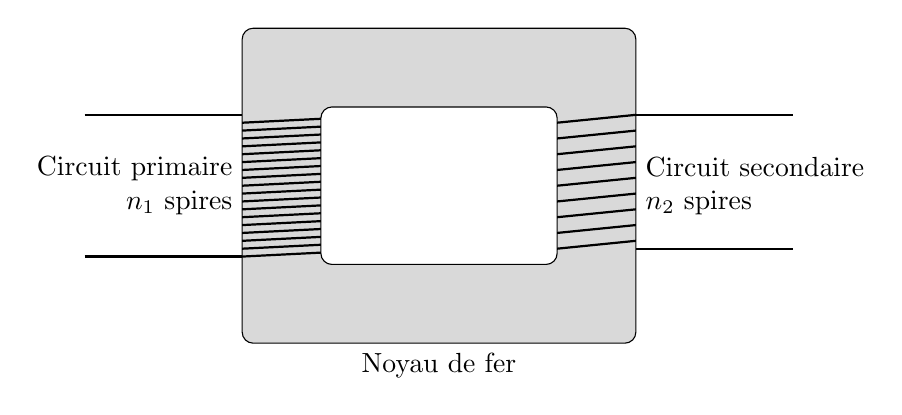
\begin{tikzpicture}
  %tikz induction
    \draw[fill=gray!30, rounded corners] (0,0) rectangle (5,4);
    \draw[fill=white, rounded corners] (1,1) rectangle (4,3);
    %primaire
    \foreach \y in {1.1, 1.2,..., 2.8}{
      \draw[thick] (0, \y) -- (1, \y+0.05);
    }
    \draw[thick] (-2, 1.1) -- (0, 1.1);
    \draw[thick] (-2, 2.9) -- (0, 2.9);
    %secondaire
    \foreach \y in {1.2, 1.4,..., 2.8}{
      \draw[thick] (4, \y) -- (5, \y+0.1);
    }
    \draw[thick] (5, 1.2) -- (7, 1.2);
    \draw[thick] (5, 2.9) -- (7, 2.9);
    \draw (0, 2) node[left, align=right]{Circuit primaire\\$n_1$ spires };
    \draw (5, 2) node[right, align=left]{Circuit secondaire\\$n_2$ spires };
    \draw (2.5, 0) node[below]{Noyau de fer};
  \end{tikzpicture}
  \captionof{figure}{Transformateur de tension.}
\end{center}
Dans un transformateur de tension idéal, les tensions $u_1$ du primaire et $u_2$ du secondaire sont reliées par 
\begin{equation}
  \frac{u_2}{u_1} = \frac{n_2}{n_1}
\end{equation}

\item Le chauffage par induction. On place un conducteur métallique dans un champ magnétique variable, le courant induit dans le conducteur le chauffe par effet Joule. On l'utilise dans la cuisine pour chauffer le fond d'une casserole ou dans l'industrie pour chauffer des pièces métalliques (voire les faire fondre).

\begin{center}
  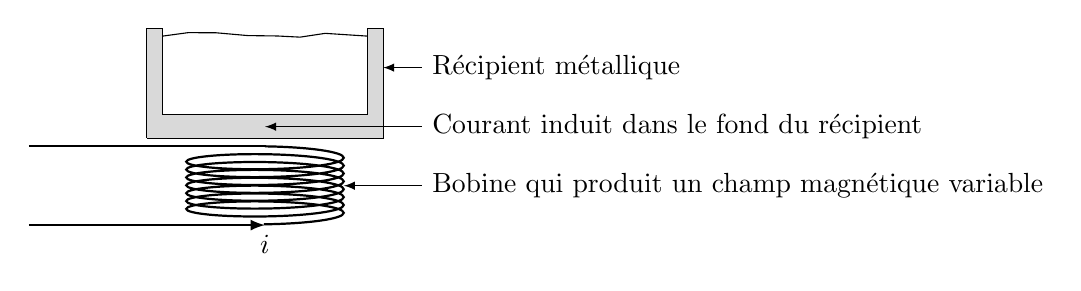
\begin{tikzpicture}
  %tikz induction
    \draw[thick,decorate, decoration={coil, amplitude=1cm, segment length=0.1cm, aspect=0.12, pre length=0, post length=0}] (0,1) -- (0,0);
    \draw[ thick] (-3, 1) -- (0,1);
    \draw[-latex, thick] (-3, 0) -- (0,0) node[below] {$i$};
    \draw[fill=gray!30] (-1.5, 1.1) -- (1.5, 1.1) -- ( 1.5, 2.5) -- (1.3, 2.5) -- (1.3, 1.4) -- (-1.3, 1.4) -- (-1.3, 2.5) -- (-1.5, 2.5) --(-1.5, 1.1);
    \draw[decorate, decoration={random steps ,amplitude=0.5mm}] (-1.3, 2.4) -- (1.3, 2.4);
     \draw[latex-] (1, 0.5) -- ++(1,0) node[right] {Bobine qui produit un champ magnétique variable};
     \draw[latex-] (1.5, 2) -- ++(0.5, 0) node[right] {Récipient métallique};
     \draw[latex-] (0, 1.25) -- ++(2, 0) node[right] {Courant induit dans le fond du récipient};
  \end{tikzpicture}
  \captionof{figure}{Chauffage d'une casserole par induction.}
\end{center}

\item On peut utiliser le phénomène d'induction pour transmettre des informations, par exemple dans les cartes sans contact RFID. Dans ce cas, le champ magnétique variable permet simultanément de fournir la puissance nécessaire au circuit électronique se trouvant dans la carte, et de transporter les informations que s'échangent la carte et le lecteur.
\end{itemize}

\end{document}
